\documentclass[11pt]{report}
\newcommand{\userName}{Rebecca Miko}
\newcommand{\institution}{University of Hertfordshire}

%Packages
\usepackage{graphicx}
\usepackage{xr}
\usepackage{hyperref}
\usepackage{geometry}
\usepackage{booktabs}

\geometry{margin=1in}

% Begin document
\begin{document}

\pagenumbering{arabic}
\begin{center}
{\Huge Progress Report}
\end{center}

\section*{Abstract}
The olfactory bulb in mammals is responsible for receiving, processing and relaying olfactory information (odours). This project investigates how naturalistic temporally fluctuating odour signals are processed and which neurons 
or neural mechanisms are able to extract information from these signals. Multiple computation models were created to represent different OB circuits between periglomerular cells and mitral cells using NEURON (Hines and Carnevale, 2006, 2001). 
The results show that the strength and frequency of these odour signals can be determined by looking at a combination of the latency and the firing rates of the output from the mitral cells. 

\section*{Research question:}
Can we predict the strength and frequency of the input by looking at two features: Firing Rates and Latency?\\

First, we look at 3 input frequencies (1, 10 and 40\,Hz) and 2 input strengths (0.315 and 0.54\,nA):
\begin{figure}[!ht]
\centering
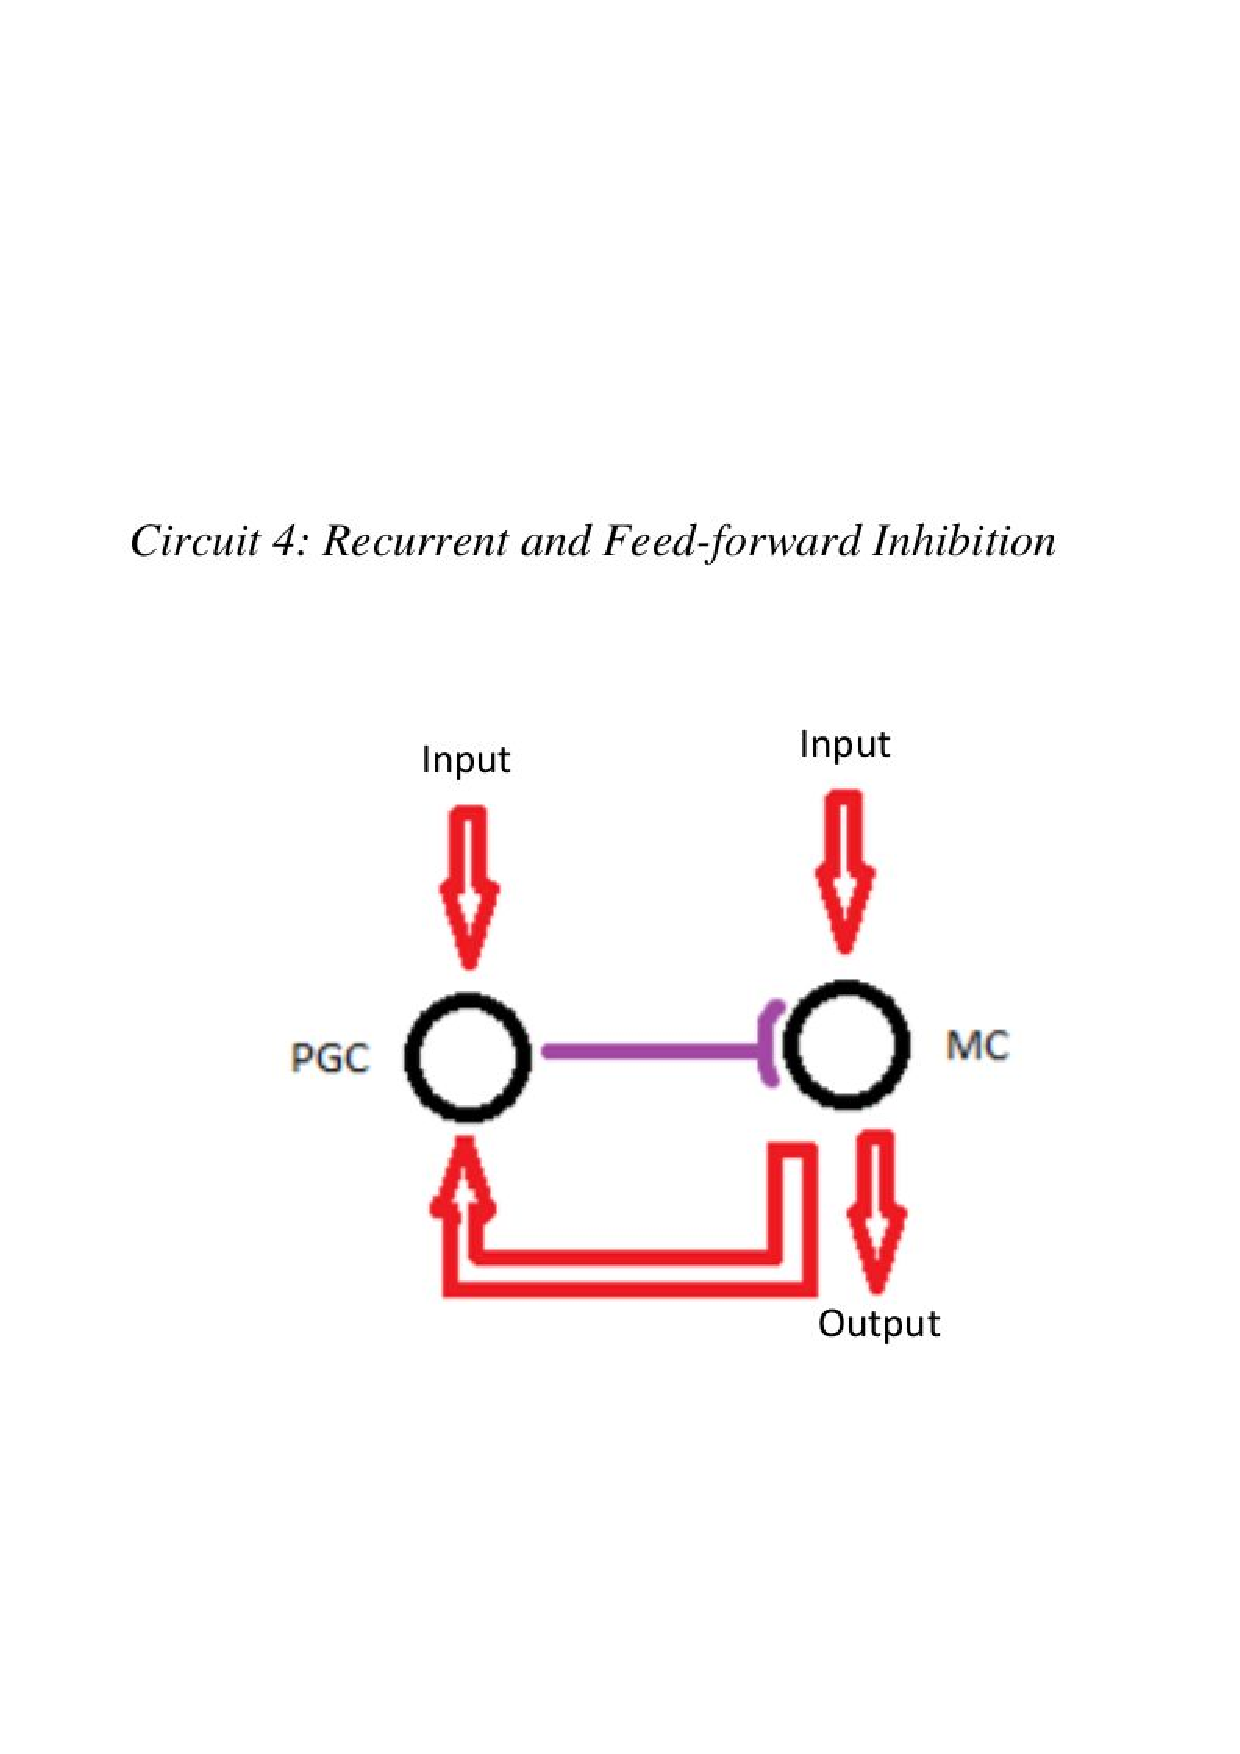
\includegraphics[trim={0 6cm 0 8cm},clip, scale=0.5]{Figures/Circuit_4.pdf}
\caption{The full model.}
\label{fig:Circuit_4}
\end{figure} 

Figure \ref{fig:Circuit_4} shows the full model (denoted as circuit 4). The PGC (periglomerular cell) and the MC (mitral cell) both recieve input, both the feed-forward and recurrent inhibition is considered, and the output from the MC is analysed. 
\newpage

\begin{figure}[!ht]
\centering
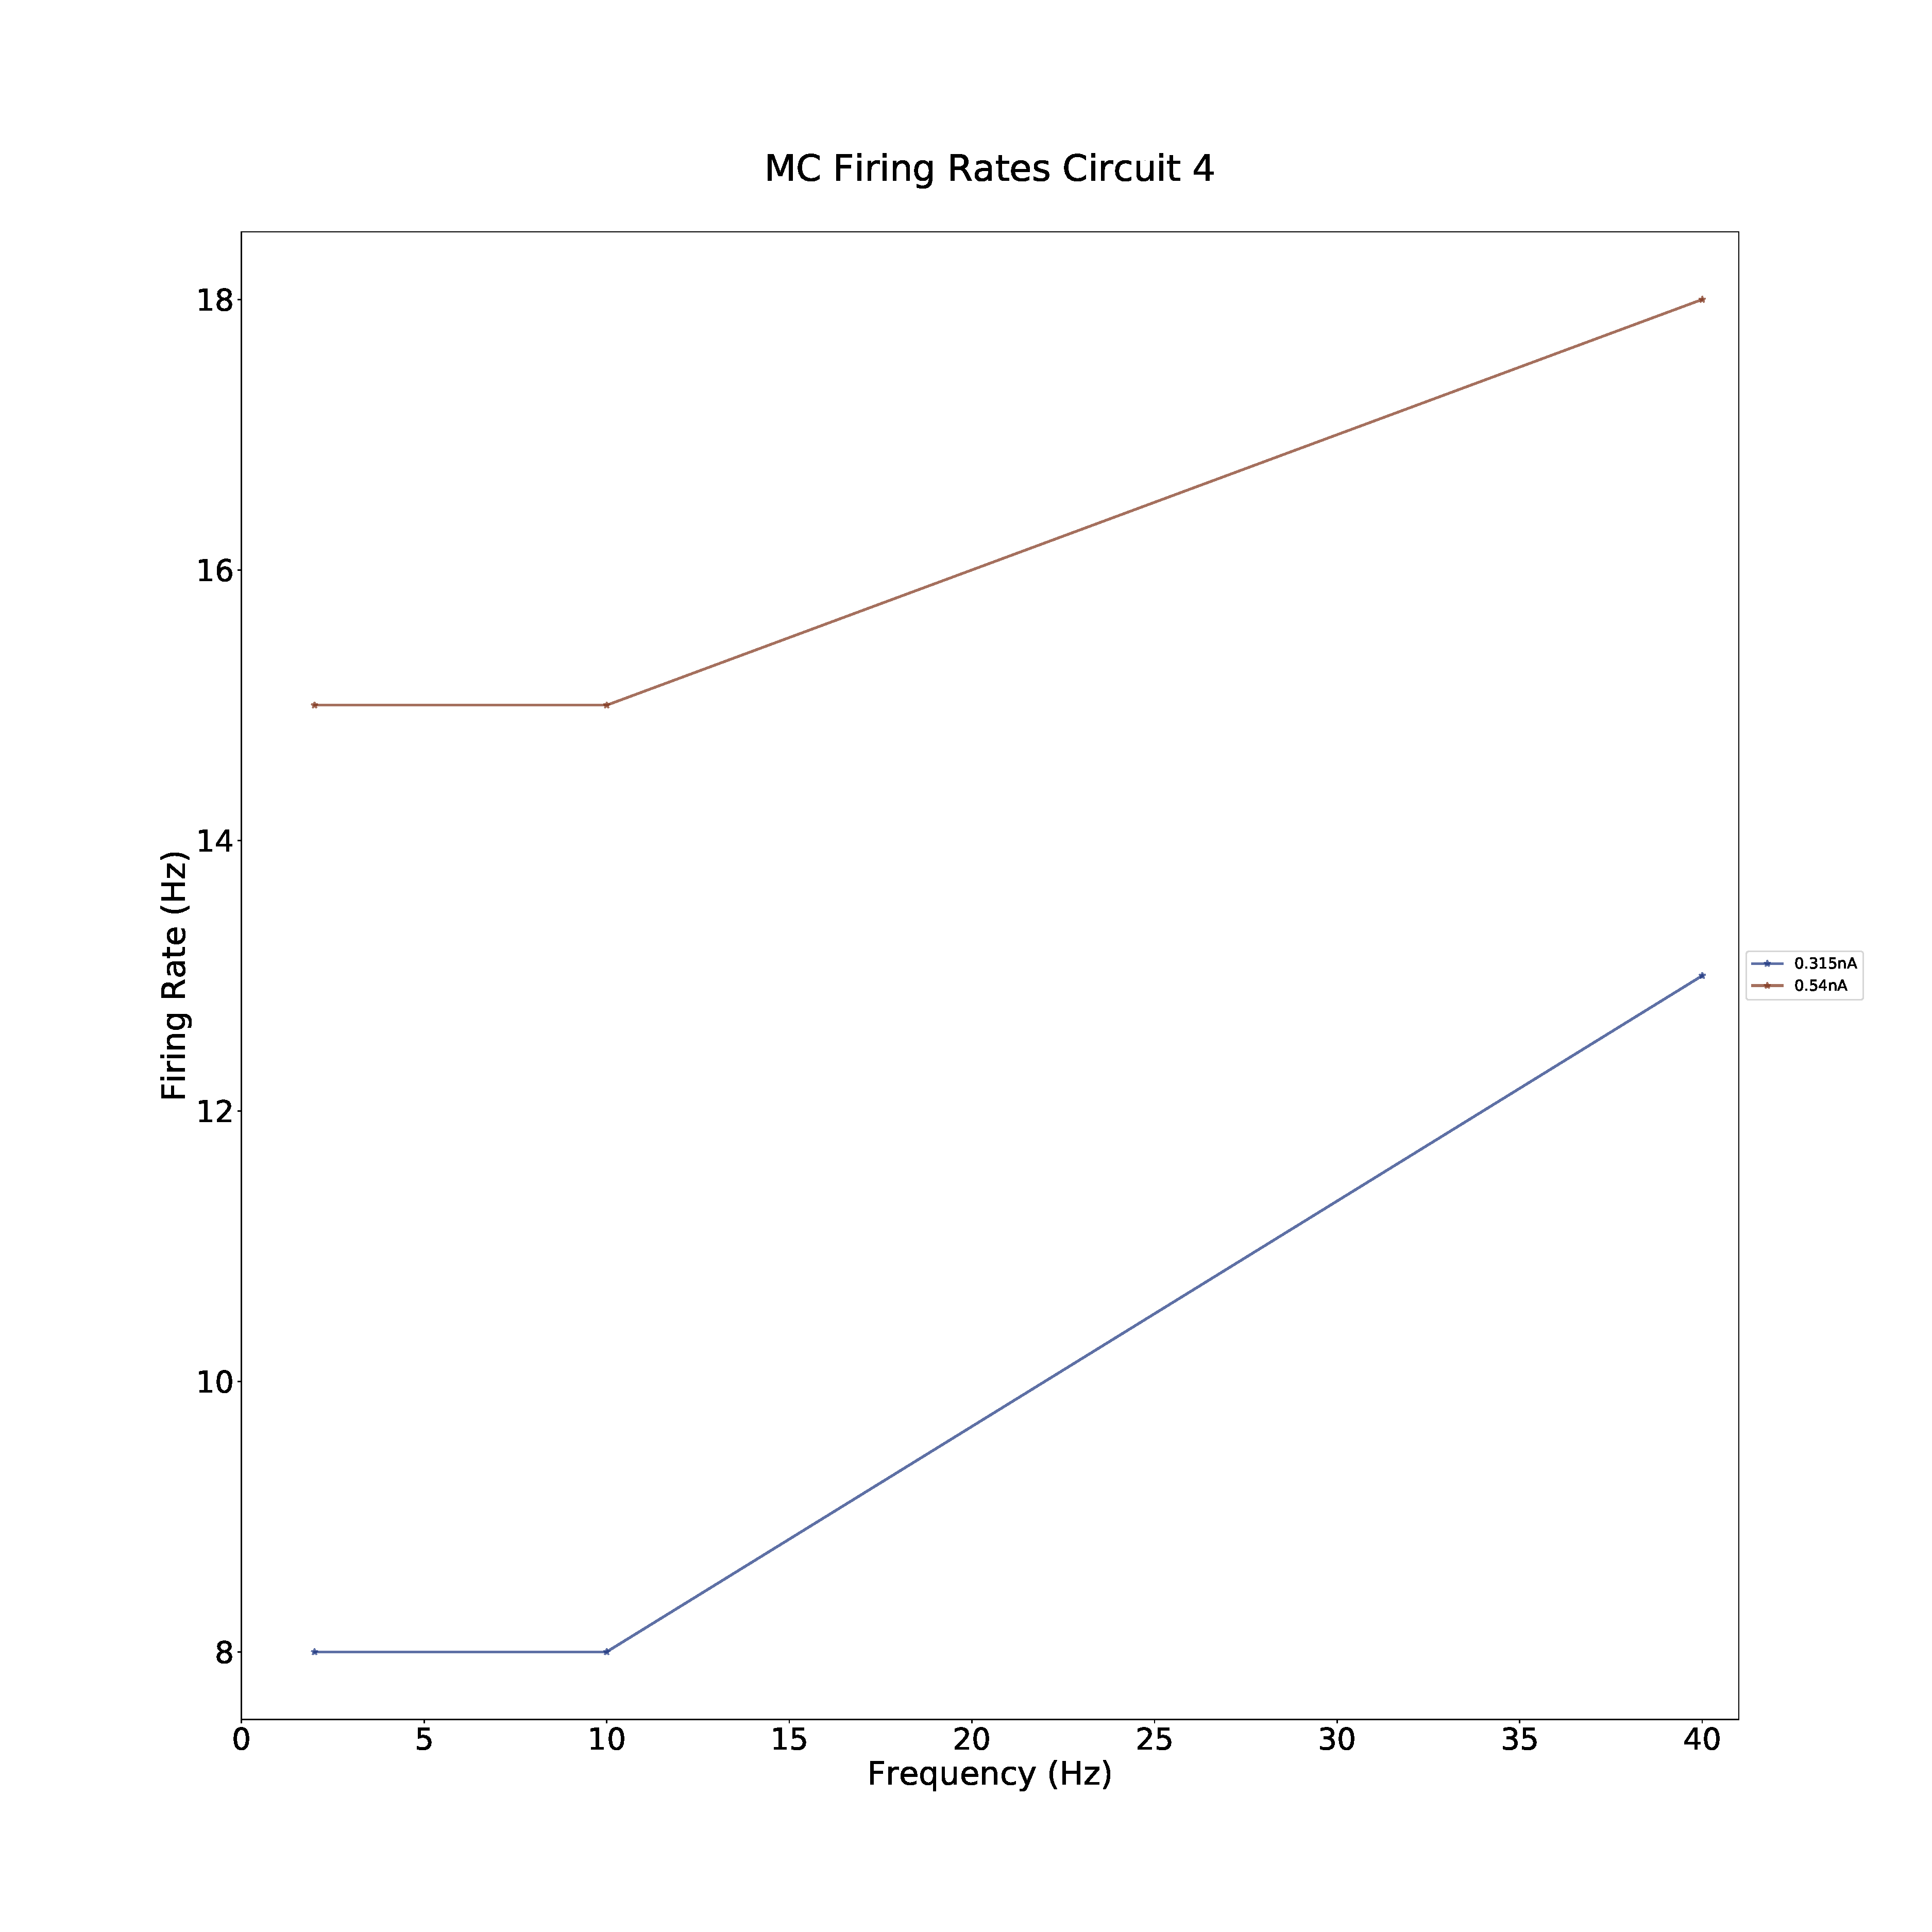
\includegraphics[scale=0.3]{Figures/MC_firing_rate_C4.pdf}
\caption{The mitral cell firing rates for circuit 4.}
\label{fig:MC_FR_C4}
\end{figure} 

In figure \ref{fig:MC_FR_C4}, it is clear that the firing rates can be used to determine the strength of the input current. However, the frequency of the input current is still unclear. 
\newpage

\begin{figure}[!ht]
\centering
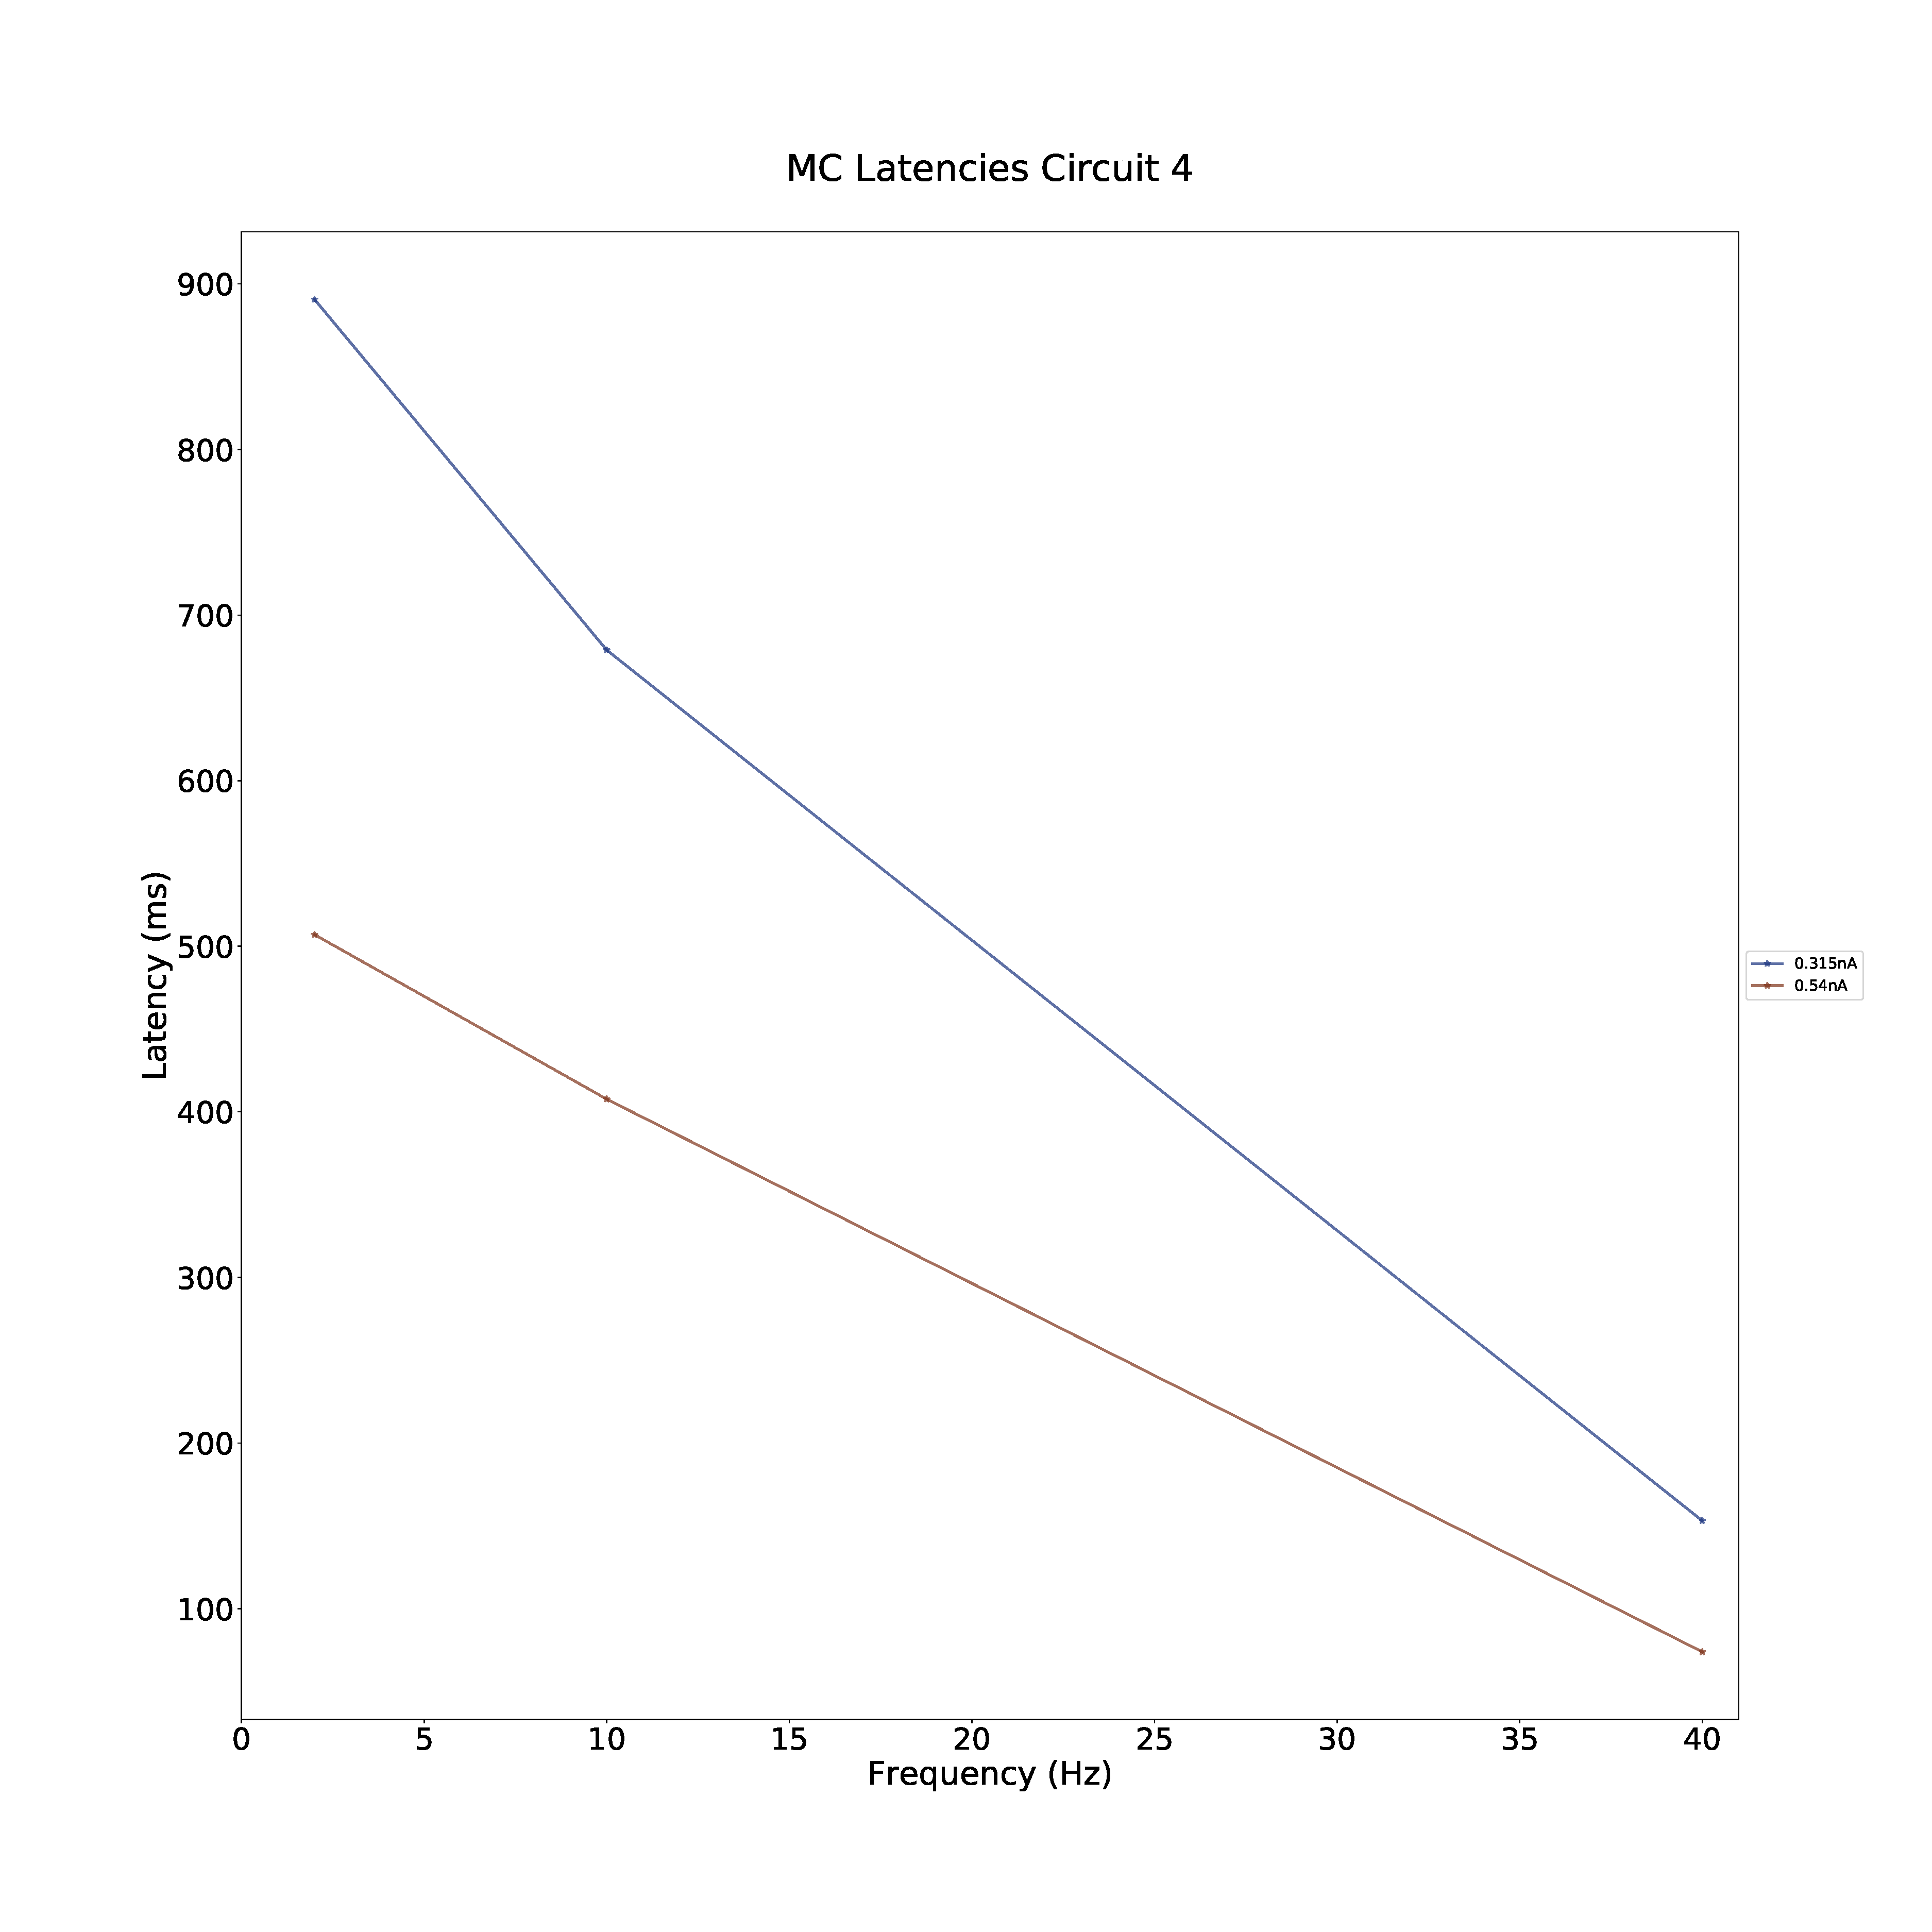
\includegraphics[scale=0.3]{Figures/MC_latencies_C4.pdf}
\caption{The mitral cell latencies for circuit 4.}
\label{fig:MC_L_C4}
\end{figure} 

Figure \ref{fig:MC_L_C4} shows that we can determine the frequency of the input from the latencies, if we know the strength of the input. Therefore, we can predict the strength and frequency of the input by looking at a combination of both firing rates and latency.

\paragraph{Underlying Mechanisms}
The strength and frequency of the input can be predicted by looking at the firing rates and latency, as described above. What mechanism is responsible for these results?

\begin{figure}[!ht]
\centering
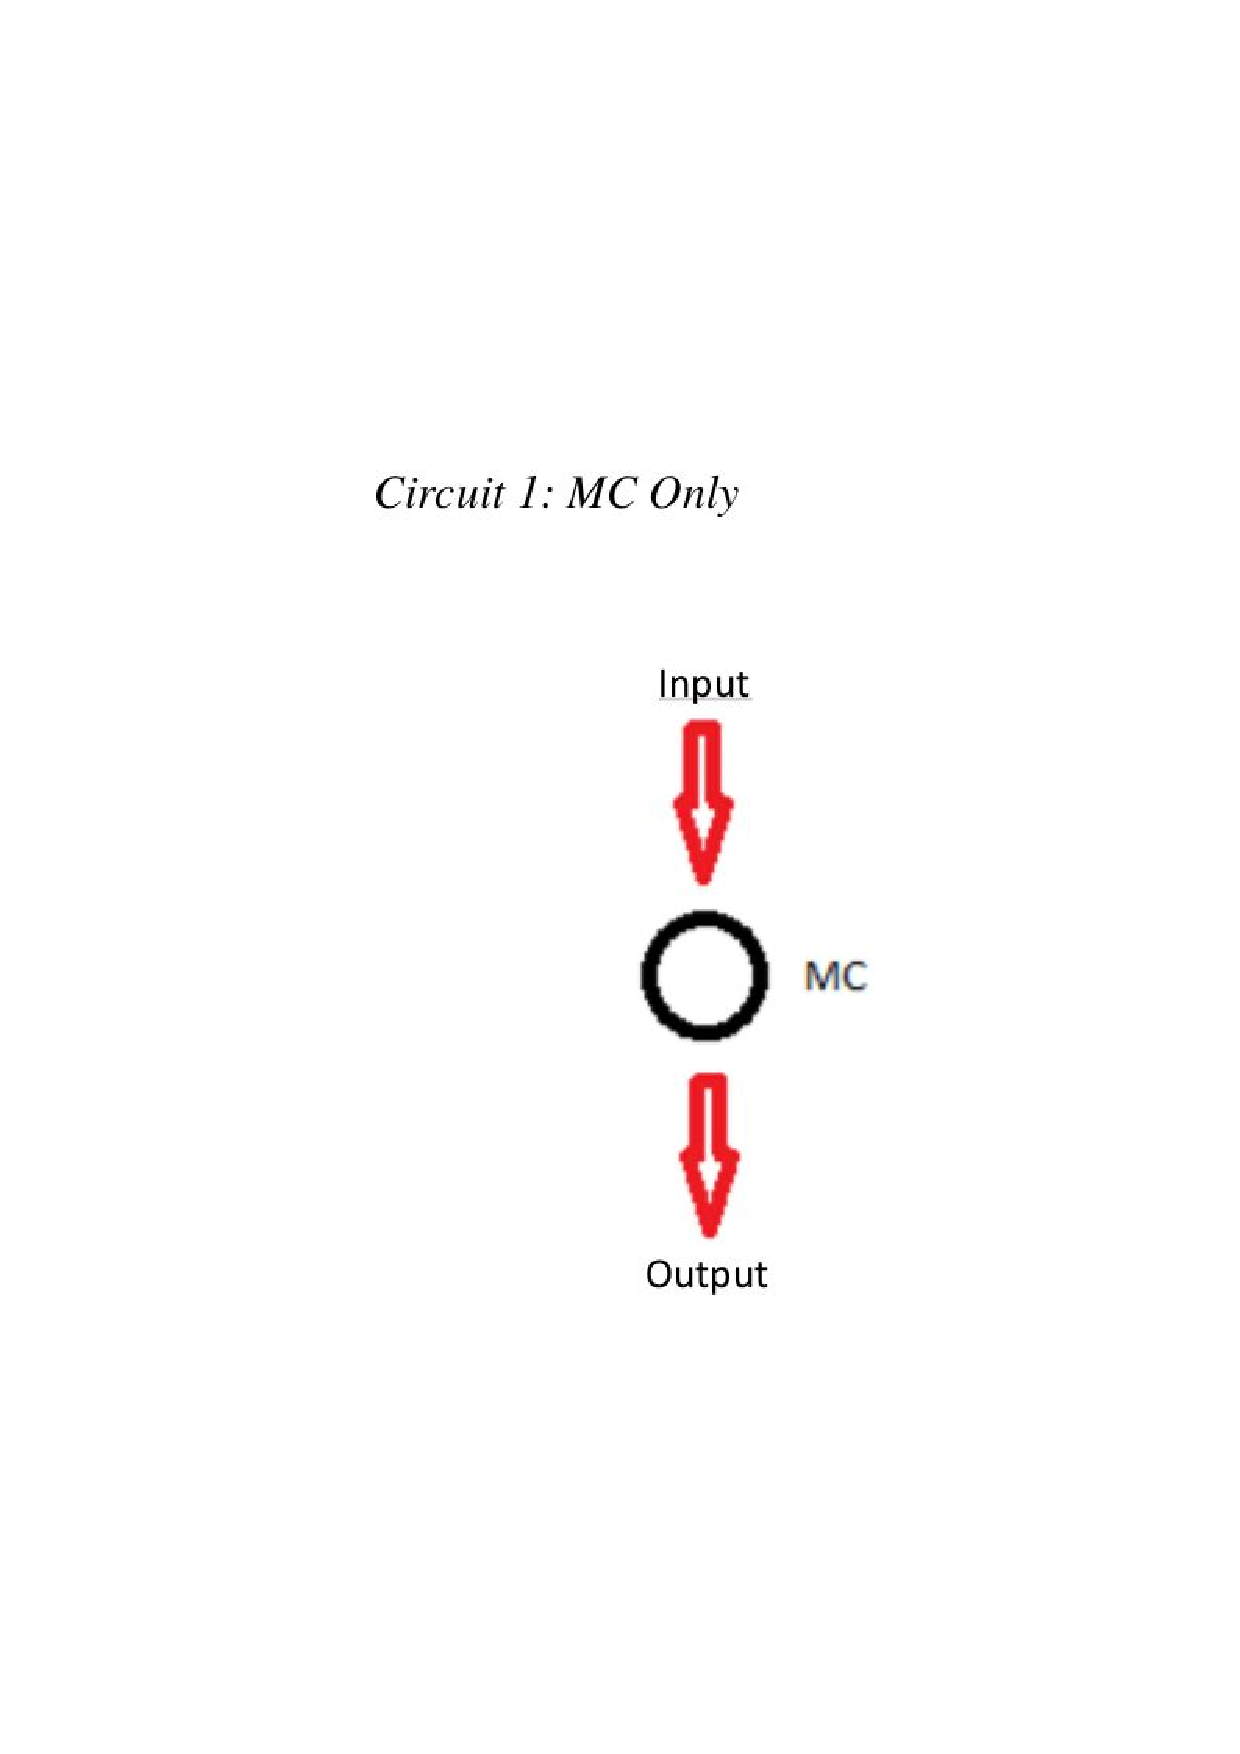
\includegraphics[trim={0 6cm 0 8cm},clip, scale=0.5]{Figures/Circuit_1.pdf}
\caption{Circuit 1. This focuses on the mitral cell only.}
\label{fig:Circuit_1}
\end{figure} 

\begin{figure}[!h]
\centering
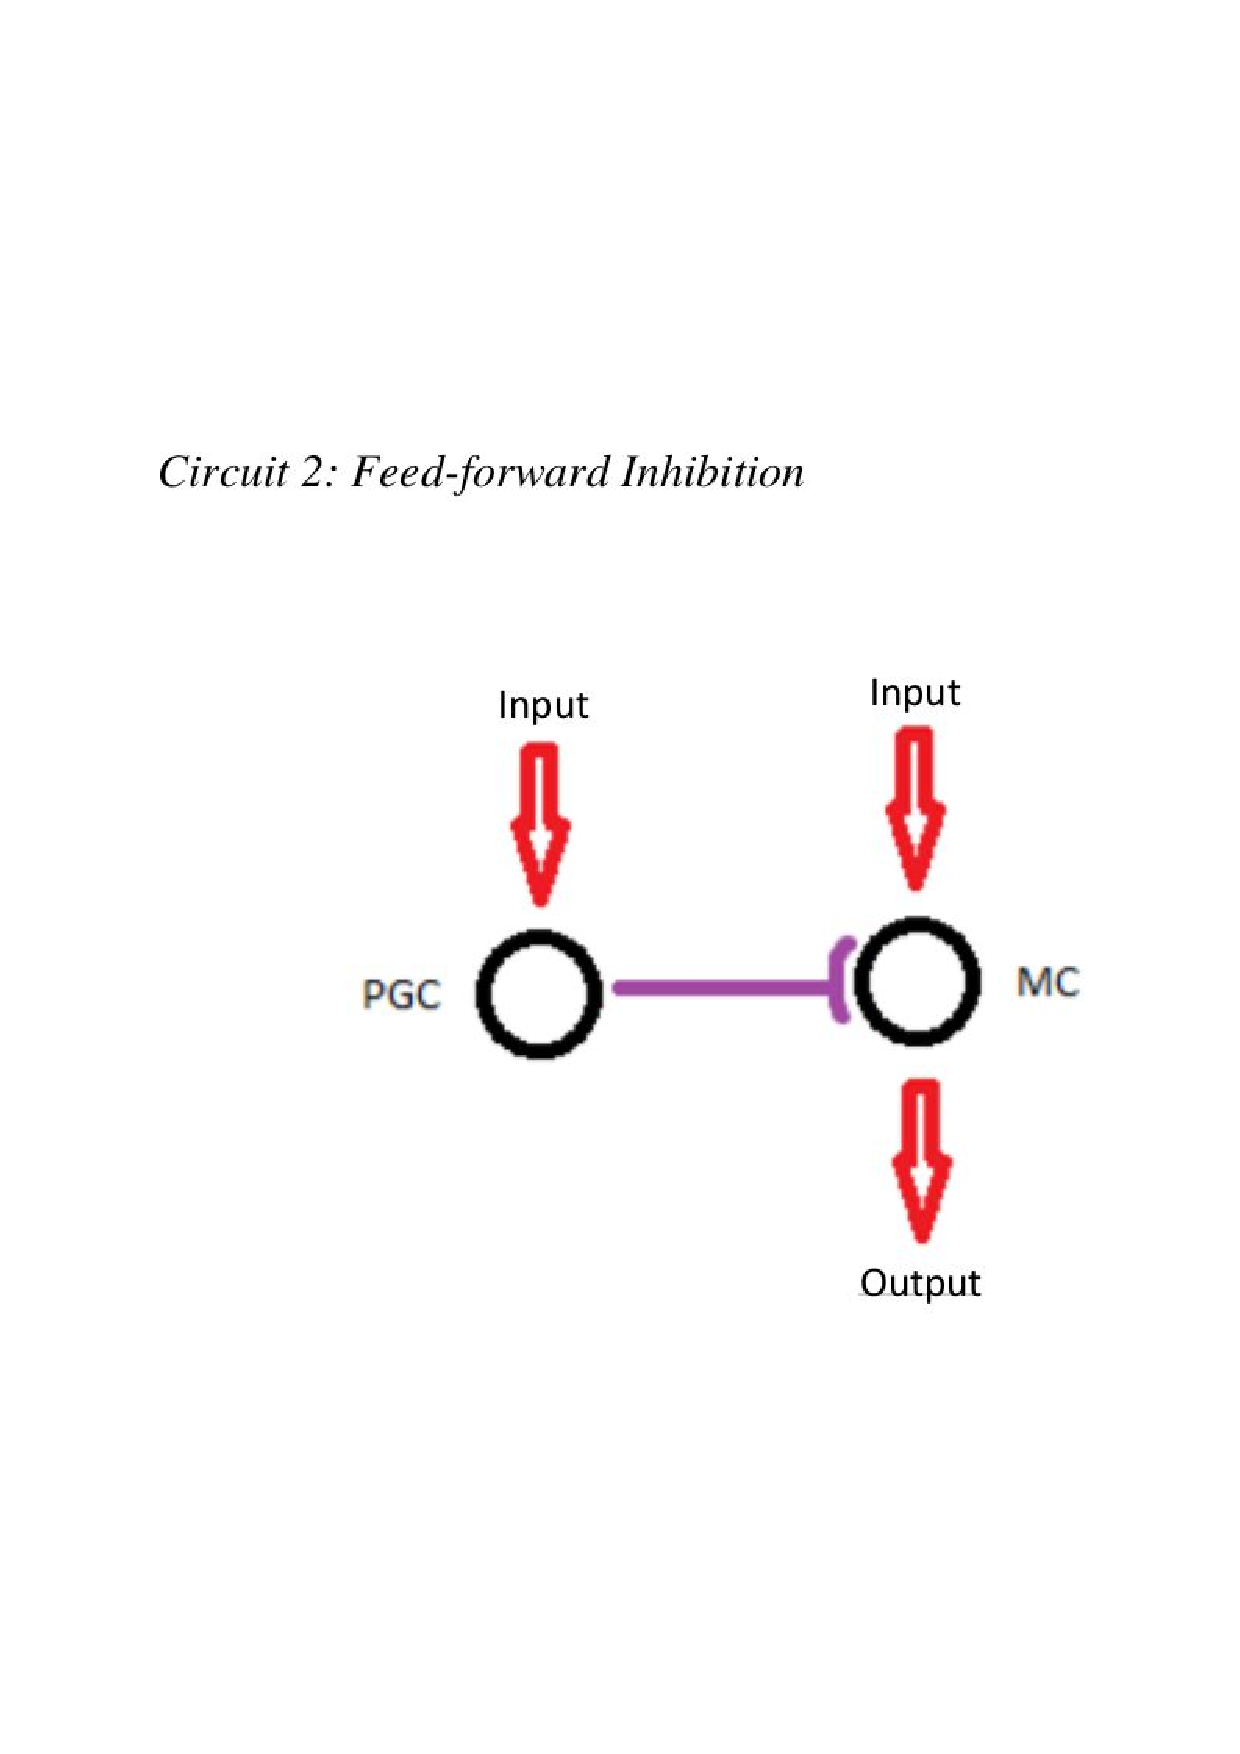
\includegraphics[trim={0 6cm 0 6cm},clip, scale=0.5]{Figures/Circuit_2.pdf}
\caption{Circuit 2. This focuses on the feed-forward inhibition.}
\label{fig:Circuit_2}
\end{figure} 
\newpage

\begin{figure}[!ht]
\centering
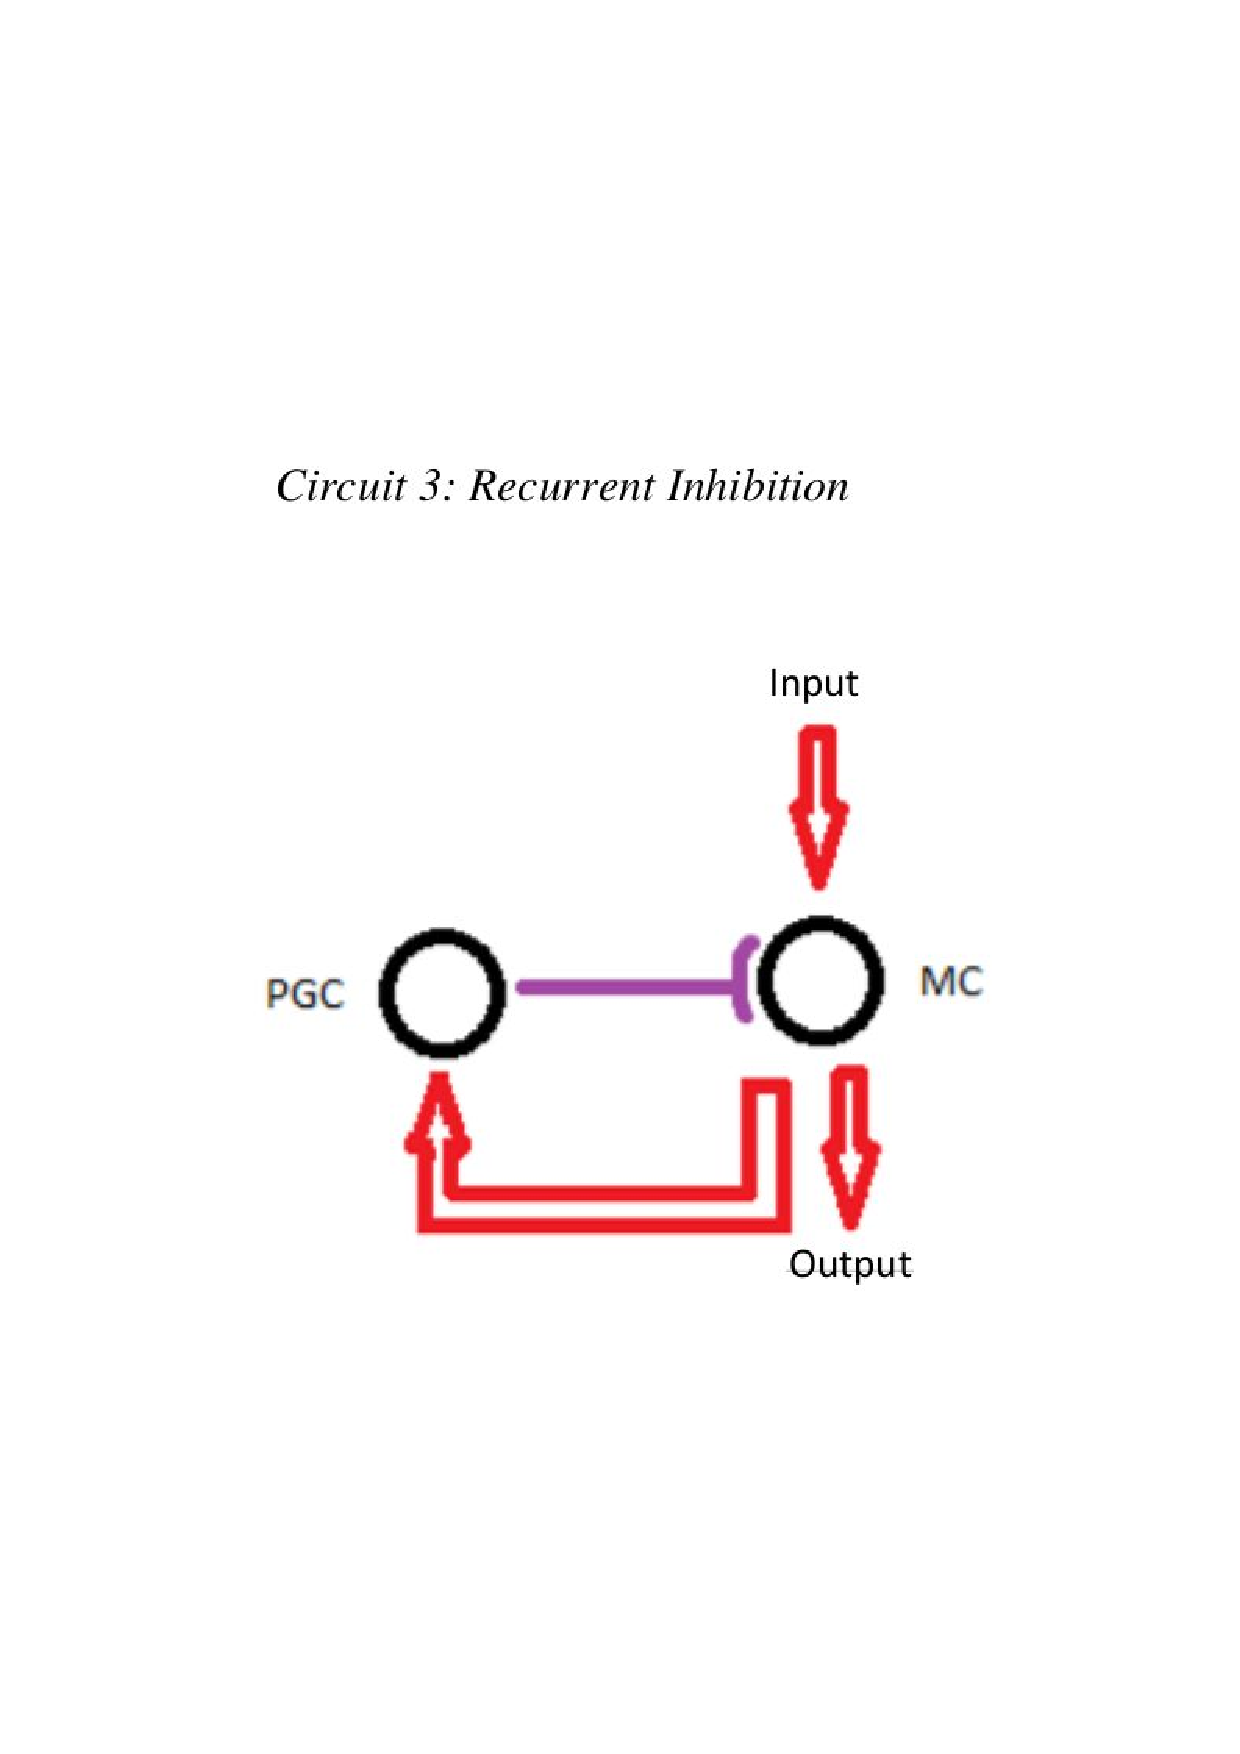
\includegraphics[trim={0 6cm 0 6cm},clip, scale=0.5]{Figures/Circuit_3.pdf}
\caption{showing circuit 3. This focuses on the recurrent inhibition.}
\label{fig:Circuit_3}
\end{figure} 

Each aspect of the model was analysed individually, see figures \ref{fig:Circuit_1}, \ref{fig:Circuit_2} and \ref{fig:Circuit_3}. Therefore, we can determine which mechanism is responsible for results found in figures 2 and 3.
\newpage

\begin{figure}[!ht]
\centering
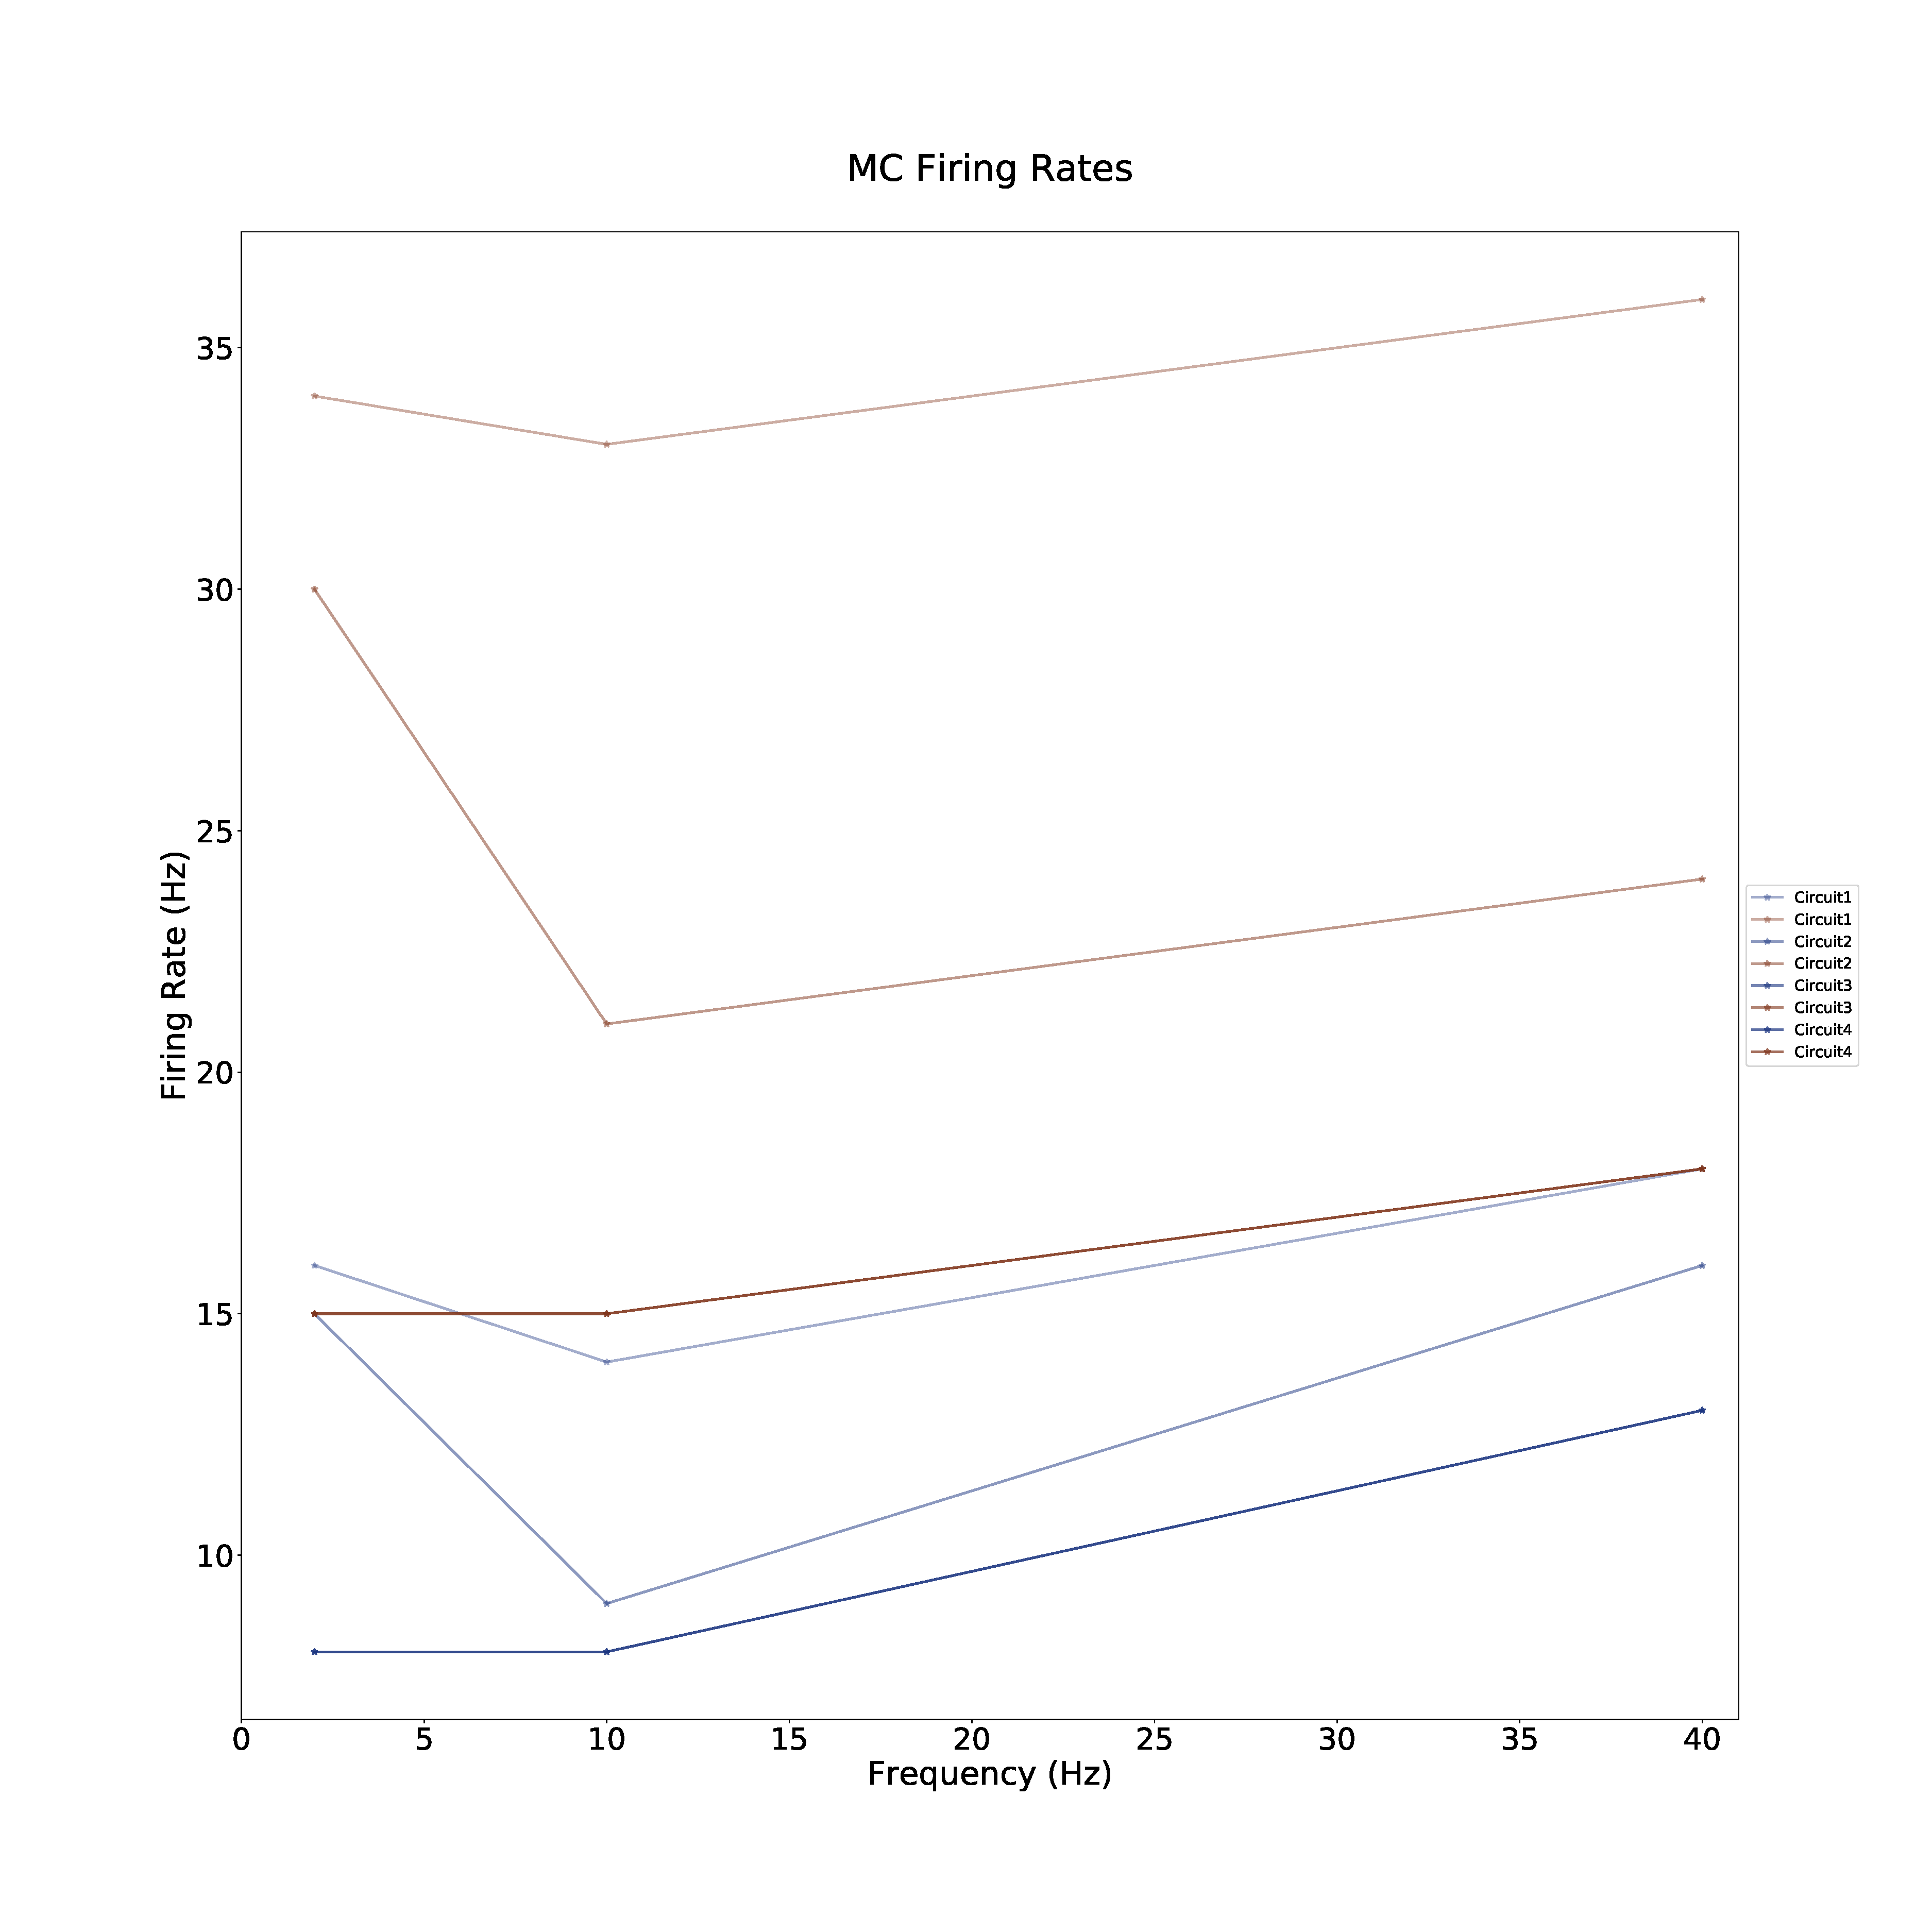
\includegraphics[scale=0.3]{Figures/MC_firing_rate.pdf}
\caption{showing the mitral cell firing rates for all circuits.}
\label{fig:MC_FR_AllC}
\end{figure} 

\begin{figure}[!ht]
\centering
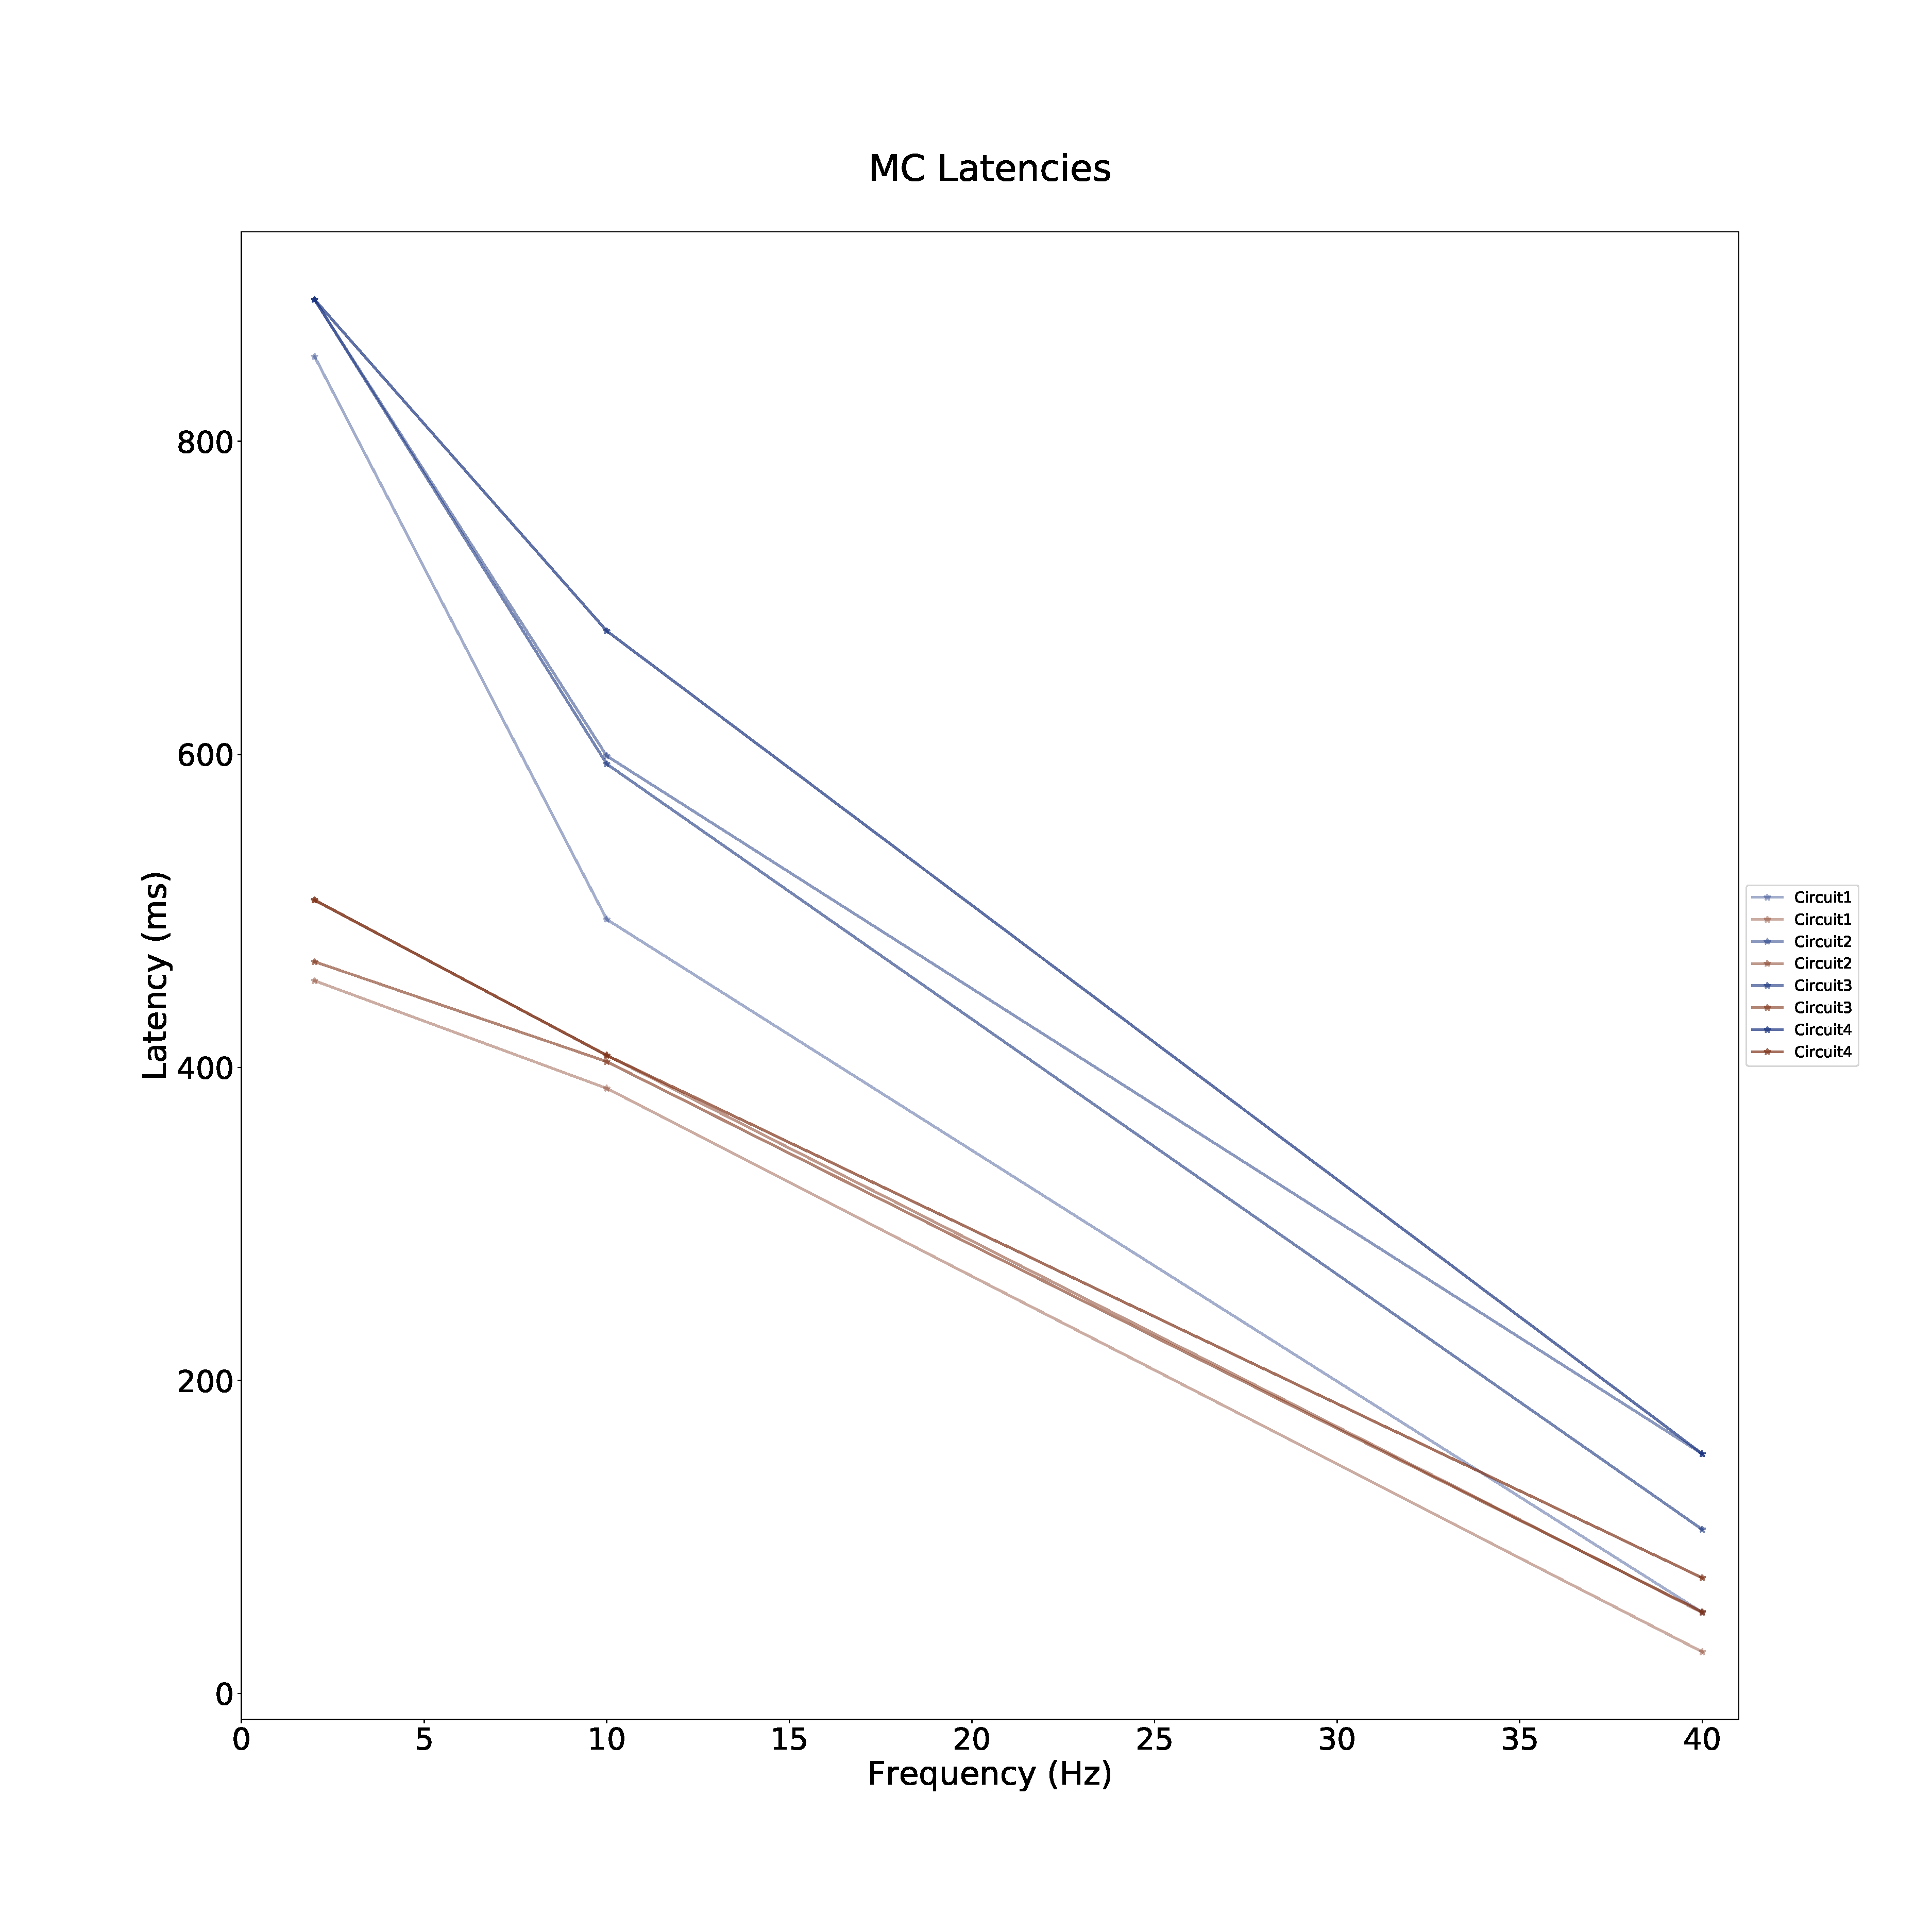
\includegraphics[scale=0.3]{Figures/MC_latencies.pdf}
\caption{showing the mitral cell latencies for all circuits.}
\label{fig:MC_L_AllC}
\end{figure}

The 'frequency-independence' of the firing rates as well as the inverse proportionality of input frequency and latency already holds for the MC only circuit (circuit 1) \ref{fig:Circuit_1}. Therefore, for these very simplistic inputs, the intrinsic mechanisms of the mitral cells are enough and none of the inhibitory circuits is needed.

\section*{Prediction}
The next step was to quantitatively consider the prediction of input strength and frequency. Therefore, 49 different combinations of strength and frequency were simulated, which were generated from 7 strengths: 0.27,0.315,0.36,0.405,0.45,0.495,0.6 ; and 7 frequencies: 1,2,5,10,20,30 and 40\,Hz). The mean firing rate and the latencies from the MC responses were extracted.

\begin{figure}[!ht]
\centering
\includegraphics[width=\textwidth]{Figures/MC_Soma_firing_rate_circuit_4}
\caption{Firing rate vs input frequency plot.}
\label{fig:frate-freq}
\end{figure}

Figure \ref{fig:frate-freq} is a plot of firing rate against frequency, which shows that the firing rate is almost independent from the input frequency.

\begin{figure}[!ht]
\centering
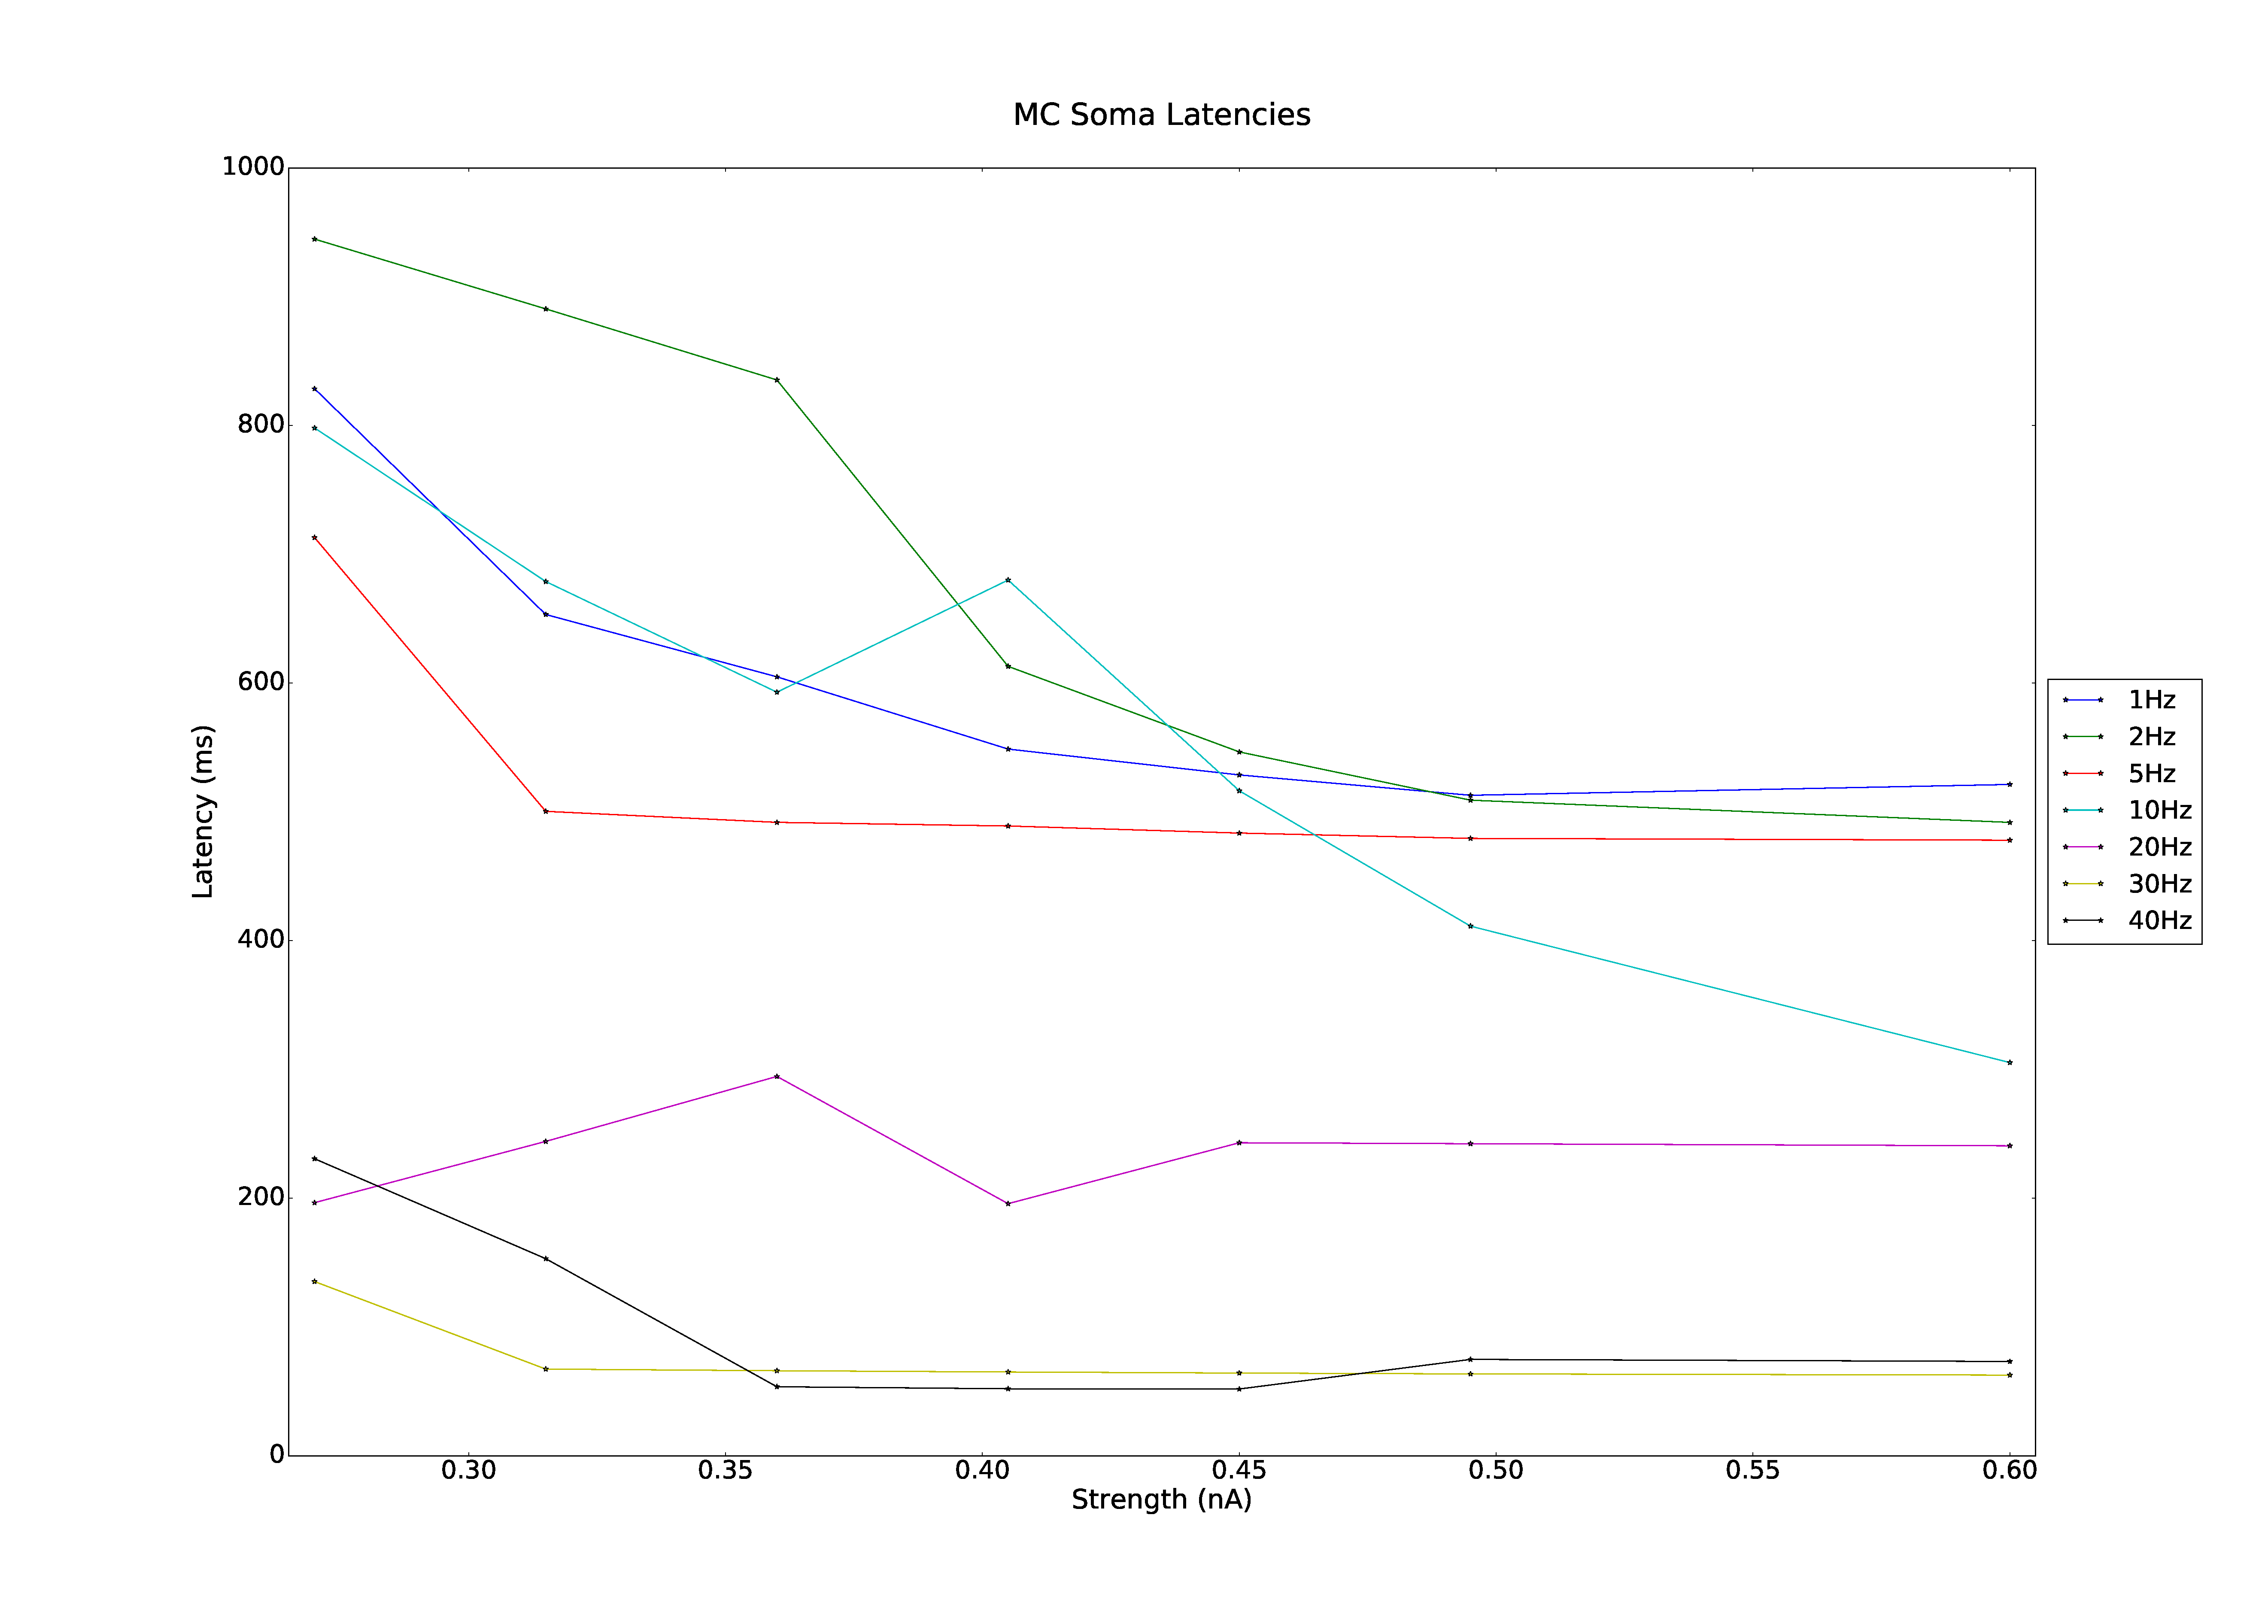
\includegraphics[width=\textwidth]{Figures/MC_Soma_latencies_vs_strength_circuit_4}
\caption{Latency vs input strength plot.}
\label{fig:lat-strength}
\end{figure}

Furthermore Figure \ref{fig:lat-strength} is a plot of latency against input strength, which shows that the latency seems only to depend on the frequency and not on the strength.

Thus, as the first and simplest predictor, the two linear functions are fitted to the data, which relate the input strength to firing rate and input frequency to latency, respectively.

\[
 FR(s) = 32.26\cdot s - 0.59
\]

and 

\[
 L(f) = -16\cdot f + 645.4
\]

Inital test of the predictor:\\
We predict the firing rate (FR) and the latency (L), for two pairs of input strength and frequency: (0.5\,nA,13\,Hz) and (0.3\,nA,1.7\,Hz).
The predictions received: FR=15.5\,Hz and L=437.4\,ms in the first case and  FR=9.1\,Hz and L=618.2\,ms in the second.
The actual results from the simulations are: FR=13.5\,Hz and L=475.6\,ms and FR=7.7\,Hz and L=711.1\,ms, respectively.

For a more detailed test, 25 new pairings of strength (range:0.15-0.7) and frequency (range:0.5-50), predict firing rate and latency, and compare them to the actual simulation results.
The root mean squared error (RMSE) is calculated for firing rate and latency:

\[
 RMSE(x^{pred},x^{act})=\sqrt { \sum_i (x^{pred}_i - x^{act}_i)^2}
\]

The values used for strength and frequency were all combinations of the following 5 different values for strength [0.3,0.32,0.35,0.58,0.6] and the 5 different values for frequency [5.78,8.21,15.53,31.98,33.17]. The RMSE for latency and firing rate are shown in Table \ref{tab:rmse}.

\begin{table}[!h]
\centering
\caption{RMSE for latency and firing rate for the 4 different circuits.}
\begin{tabular}{lcccc}
\toprule
&Circuit1&Circuit2&Circuit3&Circuit4\\
\midrule
Latency&93.2&145.6&81.3&145.5\\
Firing rates&13.8&7.36&3.2&3.4\\
\bottomrule
\end{tabular}
\label{tab:rmse}
\end{table}

However, the aim is to predict strength and frequency of the input from the 'measured' firing rates and latencies. Therefore, the invert of the two functions are shown bellow, which relate frequency to larency and firing rate to strength, respectively.

\[
s = \frac{FR+0.59}{32.26}
\]

\[
f = -\frac{L-645.4}{16}
\]

Therefore, 25 test data points from above can be used to predict strength and frequency from the measured latencies and firing rates. They can then be compared to the ground truth. This is shown in \ref{tab:rmse-inverse} bellow:

\begin{table}[!h]
\centering
\caption{RMSE for latency and firing rate for the 4 different circuits.}
\begin{tabular}{lcccc}
\toprule
&Circuit1&Circuit2&Circuit3&Circuit4\\
\midrule
Strengths&0.4&0.2&0.1&0.1\\
Frequencies&5.8&9.1&5.1&9.1\\
\bottomrule
\end{tabular}
\label{tab:rmse-inverse}
\end{table}



\end{document}